\section{Multi-View Incremental Segmentation of 3-D Point Clouds for
Mobile Robots}\label{header-n915}

\emph{IEEE ROBOTICS AND AUTOMATION LETTERS, VOL. 4, NO. 2, APRIL 2019}
{[}31{]}

\subsection{Introduction}\label{header-n917}

Mobile robots are frequently used to autonomously explore and survey
unknown areas. To understand an environment, a robot can use a 3D sensor
to acquire data in point cloud form. A point cloud is an array of 3D
points containing geometric and optionally color information. This type
of data can be used for many different purposes, the one treated in this
work is the semantic segmentation of the environment. The initial
approaches used to perform point cloud segmentation are
clustering-based. Clustering methods usually rely on generating seed
points, and subsequently, create a point cloud cluster around it. The
point can be grouped considering different features, like distance
and/or color. On the other hand, classification of point cloud data can
be carried out: in this way each point has an individual label. Some
methods project the 3D point cloud into a 2D form and perform
segmentation on the resulting image. Other methods use 3D convolutions
and others use both geometrical and scene features. Further advancements
to this line of work use, recurrent networks, or coarse-to-fine
hierarchies to incorporate neighborhood information and local
dependencies to the prediction stage. However, these methods operate on
point clouds one at a time and do not incorporate information from new
scans or they are performed offline after complete point cloud data is
obtained. In particular, semantic segmentation is usually performed on
individual scans or performed offline after complete scan data is
collected. To overcome these shortcomings, this study proposes a
multi-view incremental segmentation method that can perform online
instance segmentation of 3D point clouds. A neural network assigns a
label to each point and the segmentation results are progressively
updated. The key idea is to consider a select few of the previous scans,
to improve the segmentation of the current scan.

\subsection{Proposed method}\label{header-n919}

The test and training data are obtained from the Stanford 3D Indoor
Spaces (S3DIS) dataset. In contains 6 building areas with point clouds
segments individually annotated. It also contains 13 classes of objects,
like walls, chairs, doors, and other types of furniture. A virtual robot
with laser scanners is placed in the environment and acquires laser
scans by ray-tracing. The robot is also equipped with cameras so that
color information can be mapped onto the point cloud. The robot acquires
a scan every $2m$ and ray-tracing is carried out. The figure below
shows the original point cloud of a room as well as the resulting point
cloud obtained by ray-tracing along a trajectory.

\begin{figure}[h!]
\centering
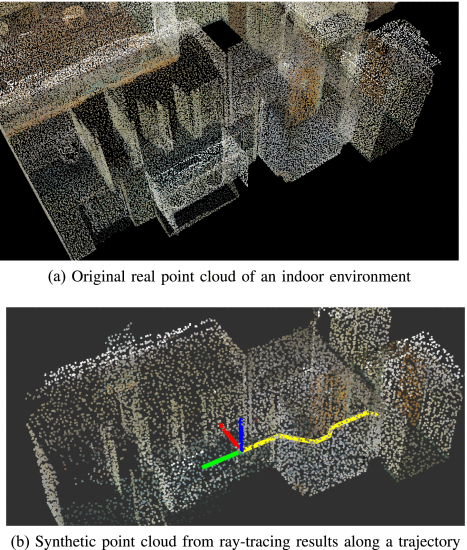
\includegraphics[width=0.7\linewidth]{images/pointclouds.png}
\caption{Visualization of dynamic scanning by ray-tracing for a virtual mobile robot}
\end{figure}

The proposed incremental segmentation method involves a neural network
architecture, named Multi-view Context Pooling Network (MCPNet), that
jointly predicts an instance label and a class label for each scanned
point. The class label describes the semantic class of a point (i.e.
wall, door, table, etc.) whereas the instance label is a unique ID such
that only points from the same object instance have the same ID. In an
online segmentation procedure, it is important to keep track of newly
scanned points and their relationship to previously scanned points.
Thus, a voxel grid with a grid size of $0.1m$ is used as a lookup
table to store the point coordinates and their corresponding
segmentation results: the point cloud is limited to one point per voxel.
First, each input scan considers as a valid point only those in an area
of radius $2m$ around the robot (points discarded will be considered
in future scans). Next, the point coordinates are normalized so that the
x-y coordinates are centered around the robot and the z-coordinate is
zero at the floor level. The points are then divided into batches of
$N\times 6$ matrices, where $N$ is the batch size and the columns
are X-Y-Z-R-G-B values. These matrices are passed to the network.
MCPNet's architecture is reported in the following figure.

\begin{figure}[h!]
\centering
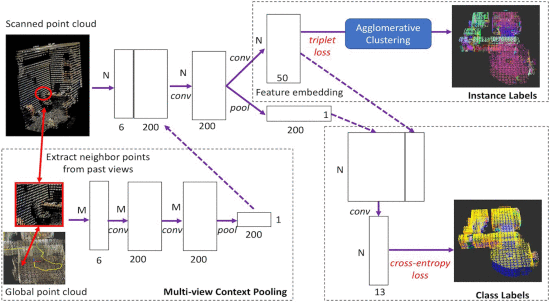
\includegraphics[width=0.91\linewidth]{images/MCPNetarc.png}
\caption{MCPNet architecture for incremental instance segmentation of 3D point clouds}
\end{figure}

The input matrix is first passed through a 1D convolution layer to form
an intermediate $N\times 200$ feature matrix. The network then splits
into two branches: the lower branch for classification and the upper
branch for clustering. The \emph{lower branch} uses a max-pooling
function to compute a global feature vector representing the input
points. This is then concatenated with the feature embedding from the
upper branch and passed through another 1D convolution layer to compute
class probabilities for each point, represented as a $N\times 13$
matrix since there are 13 classes. The \emph{upper branch} aims to
project the point features to an embedding space that is suitable for
clustering. This is enforced by computing a triplet loss between sets of
three points, $p_1$ , $p_2$ which originate from the same object and
$p_3$ which originates from a different object and minimizing the
resulting loss function (the projection is a function
$f : \R^{3} \rightarrow \R^{50}$). At training time, minimizing the
triplet loss encourages the distance between points that should belong
to the same object to be greater than that of points that should belong
to different objects in the embedding space, i.e.
$\parallel f(p_1) - f(p_2)\parallel^{2} + \alpha < \parallel f(p_1) - f(p_3)\parallel^{2}$,
where $\alpha$ is the margin parameter. At inference time, fo each
point $p_i$ a set of neighbor points are retrieved (points that is at
most one cell away from $p_i$). Then, each point $p_i$ is only
connected to a neighboring point $p_j$ if the cosine similarity
\newline
$\frac{f(p_i) \cdot f(p_j)}{\parallel f(p_i)\parallel \parallel f(p_j)\parallel}$
\newline
is greater than $\beta$ (a preset threshold). The following rules are
then applied:

\begin{itemize}
\item
  if no connections exist, the point is initialized as the seed for a
  new cluster with a new instance ID; 
\item
  if connections exist to a single existing cluster, the point is added
  to that cluster and takes the corresponding instance ID;
\item
  if connections exist to multiple existing clusters, all connected
  clusters are merged and their instance IDs are updated accordingly.
\end{itemize}

The \emph{Multi-view Context Pooling} (MCP) module incorporates
contextual information from previous views to improve the classification
accuracy. The input to the MCP module is an $N\times M\times 6$ tensor
that stores context points for each of the $N$ points in the current
input (only $M$ points from previous scans are considered). A context
point for point $p_i$ is defined as any point from previous views that
is at most three cells away from $p_i$ in the global voxel grid.

\subsection{Experiments results}\label{header-n935}

The instance segmentation results were first evaluated in terms of the
classification accuracy on the S3DIS dataset, where one area of the
dataset is held out as test data whereas the remaining areas are used as
training data. The proposed method are compared with other conventional
approaches: PointNet {[}14{]}, PointNet++ {[}32{]}, VoxNet {[}33{]} and
SGPN. The evaluation metrics are:

\begin{itemize}
\item
  \textbf{Intersection-Over-Union (IOU):} it is defined as the number of
  true positive points divided by the total true positive, false
  positive, and false negative points.
\item
  \textbf{Point-wise Accuracy:} it is the number of true positive points
  divided by the total number of points.
\item
  \textbf{Object-wise Accuracy:} defined as the number of true positive
  object instances divided by the total number of object instances.
\end{itemize}

The table below shows the results obtained.

\begin{figure}[h!]
\centering
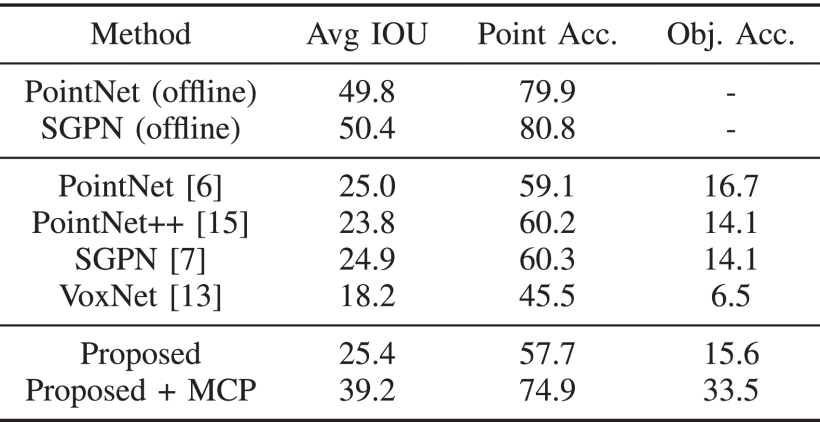
\includegraphics[width=0.7\linewidth]{images/segresultsaccu.png}
\caption{Classification accuracy on S3DIS dataset}
\end{figure}

Experimental results show that the proposed method with MCP outperforms
the other methods in terms of both IOU and accuracy. The authors
performed also an analysis of the effect of the number of the context
points used in the proposed MCP module on the classification accuracy.
The following graph shows that the average accuracy increases with
number of context points but also incurs a higher computational cost.
\newpage
\begin{figure}[h!]
\centering
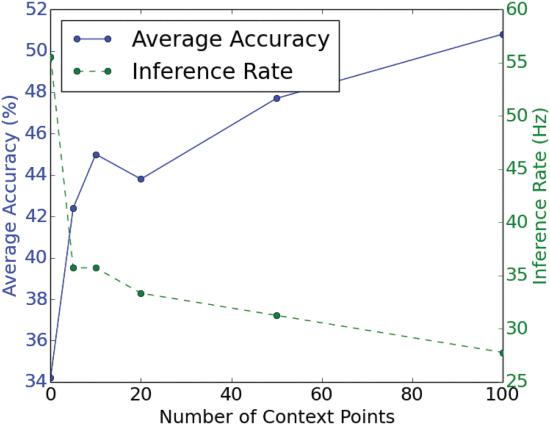
\includegraphics[width=0.7\linewidth]{images/MCPpoints.png}
\caption{Classification accuracy and inference rate as a function of the number of context points}
\end{figure}

On the other hand, the clustering performance was measured using three
different metrics: normalized mutual information (NMI), adjusted mutual
information (AMI), and adjusted rand index (ARI), as defined in
{[}35{]}. In particular, PointNet, PointNet++, and VoxNet used a
clustering technique in which connected components are formed between
points with the same class label, while the remaining methods used the
agglomerative clustering technique described in this work, with
$\beta = 0.98$ for SGPN and $\beta = 0.9$ for MCPNet. The table
below shows the results obtained.

\begin{figure}[h!]
\centering
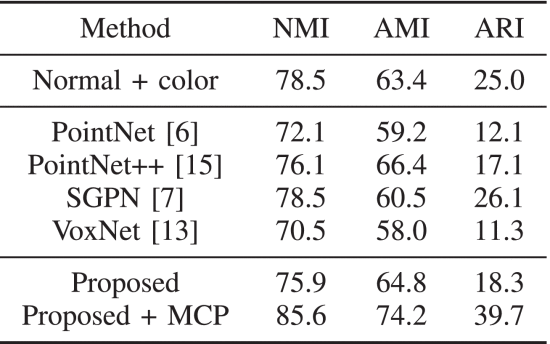
\includegraphics[width=0.65\linewidth]{images/clusper.png}
\caption{Clustering performance on S3DIS dataset}
\end{figure}

Results show that even the simple normal + color-based region-growing
scheme can achieve a good clustering, but the proposed method with MCP
achieved the best clustering result overall. The following figure shows
the global instance segmentation results at intermediate points along
the incremental scanning process: input point cloud with virtual robot
trajectory (top row), clustering results (middle row) and classification
results (bottom row).

\begin{figure}[h!]
\centering
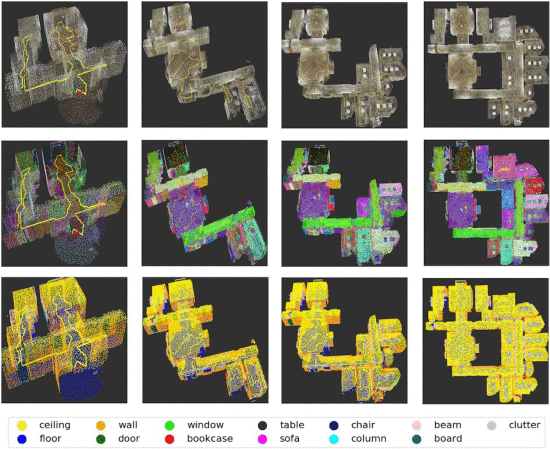
\includegraphics[width=0.7\linewidth]{images/incremseg.png}
\caption{Incremental segmentation results on S3DIS test dataset}
\end{figure}

Experimental results show that the proposed approach led to 15\%
improvement in accuracy and 7\% improvement in NMI compared to the next
best online method.